\subsection{Introduction}
This method leverages the Perspective-n-Point (PnP) problem to estimate the 3D pose of a vehicle from a single image frame. Unlike homography-based approaches, PnP allows for accurate reconstruction even when using out-of-plane points, such as the side mirror. The method is implemented in two main variants: one using 4 coplanar points (rear lights and license plate), and another using 5 points, including the mirror, to assess the impact of additional 3D depth on localization accuracy.

\subsection{Theoretical framework}
\subsubsection{The perspective-n-point problem}
The PnP problem involves estimating the position and orientation (pose) of a camera relative to a known 3D object, given:
\begin{itemize}
    \item A set of $n \geq 4$ known 3D points in the object coordinate system,
    \item Their corresponding 2D projections in the image plane,
    \item The camera's intrinsic matrix $K$.

\end{itemize}

Mathematically, the PnP problem seeks to find the rotation matrix $\mathbf{R} \in SO(3)$ and translation vector $\mathbf{t} \in \mathbb{R}^3$ that satisfy the camera projection equation:
\begin{equation}
    s \cdot \mathbf{p}_i = \mathbf{K} \cdot [\mathbf{R}|\mathbf{t}] \cdot \mathbf{P}_i
\end{equation}
where $\mathbf{p}_i$ represents the 2D image coordinates, $\mathbf{P}_i$ the corresponding 3D world coordinates, $\mathbf{K}$ the camera intrinsic matrix, and $s$ a scale factor. The rotation matrix $\mathbf{R}$ belongs to the \textit{Special Orthogonal Group} $SO(3)$, which denotes the set of all $3 \times 3$ orthogonal matrices with determinant equal to 1. This constraint ensures that $\mathbf{R}$ represents a proper rotation in 3D space, preserving lengths and angles without reflection. 

\subsubsection{PnP vs homography}
The main distinction between PnP and homography methods (\texttt{findHomography}) lies in their assumptions:
\begin{itemize}
    \item Homography assumes that all 3D points lie on the same plane (planar geometry).
    \item PnP makes no such assumption and performs well even with non-coplanar configurations. It is thus more robust in low-perspective conditions or when using points with different depths.
\end{itemize}

\subsubsection{PnP algorithm variants}
Modern PnP solvers employ different strategies for pose estimation. \textbf{Iterative PnP} methods require an initial pose estimate and refine it through non-linear optimization, typically providing higher accuracy when a reasonable initialization is available. \textbf{EPnP (Efficient PnP)} solvers, implemented through the \texttt{SOLVEPNP\_EPNP} method, compute the pose using a non-iterative approach based on expressing 3D points as weighted sums of four virtual control points. This method offers computational efficiency and numerical stability without requiring initial pose estimates, making it particularly suitable for real-time applications. \textbf{PnPRANSAC} combines pose estimation with robust outlier detection using random sample consensus, making it suitable for noisy feature correspondences where some point matches may be incorrect.

\subsection{Methodology}
\subsubsection{Four-point PnP approach: license plate and taillights}
The first methodology employs a four-point correspondence system utilizing the vehicle's license plate and taillights positions. This approach leverages the geometric regularity and predictable spatial relationships of these vehicle features to establish reliable 3D-to-2D point correspondences.
\paragraph{Feature point selection and 3D model definition}
The 3D vehicle model is defined using four key reference points:
\begin{itemize}
    \item \textbf{License plate corners}: two points representing the lower corners of the rear license plate.
    \item \textbf{Taillights points}: two points representing the rear taillights.
\end{itemize}
\paragraph{PnP solver implementation and comparison}
Two distinct PnP solving strategies were implemented and evaluated:
\begin{itemize}
    \item \textbf{Iterative PnP with initial pose estimation}: This approach first computes a rough pose estimate using analytical methods, then refines this estimate through iterative optimization. The initial pose is derived from the license plate plane geometry, providing a stable starting point for convergence.
    \item \textbf{Direct PnP solution}: This method computes the pose directly from the four-point correspondences without requiring initialization. The solver employs robust estimation techniques to handle potential noise and outliers in the feature detection process.
\end{itemize}

Experimental evaluation revealed that both approaches converge to nearly identical solutions when applied to the same feature correspondences.

\subsubsection{Five-point PnP approach: enhanced model with mirror integration}
To improve pose estimation accuracy and provide additional geometric constraints, we extended the methodology to incorporate a fifth reference point: the vehicle's side mirror position.
\paragraph{Extended 3D model definition}
The enhanced model incorporates:
\begin{itemize}
    \item \textbf{License plate corners} (2 points)
    \item \textbf{Headlight centers} (2 points)
    \item \textbf{Side mirror center} (1 point)
\end{itemize}
The addition of the side mirror point provides several advantages:
\begin{enumerate}
    \item \textbf{Geometric diversity}: the mirror point lies off the rear plane, providing depth variation
    \item \textbf{Constraint redundancy}: Additional correspondences improve pose estimation robustness
    \item \textbf{Bounding box refinement}: the mirror position enables more accurate vehicle extent estimation
\end{enumerate}

\subsection{Results and visual comparison}

Figure~\ref{fig:pnp_4pts} compares the localization results obtained using the four-point model with two different PnP solvers: the Iterative algorithm and EPnP. Both methods yield nearly identical poses and projected bounding boxes, confirming the reliability and consistency of our initial estimation of the Spose.

\begin{figure}[h]
    \centering
    \hspace*{\fill}
    \begin{subfigure}[b]{0.30\textwidth}
        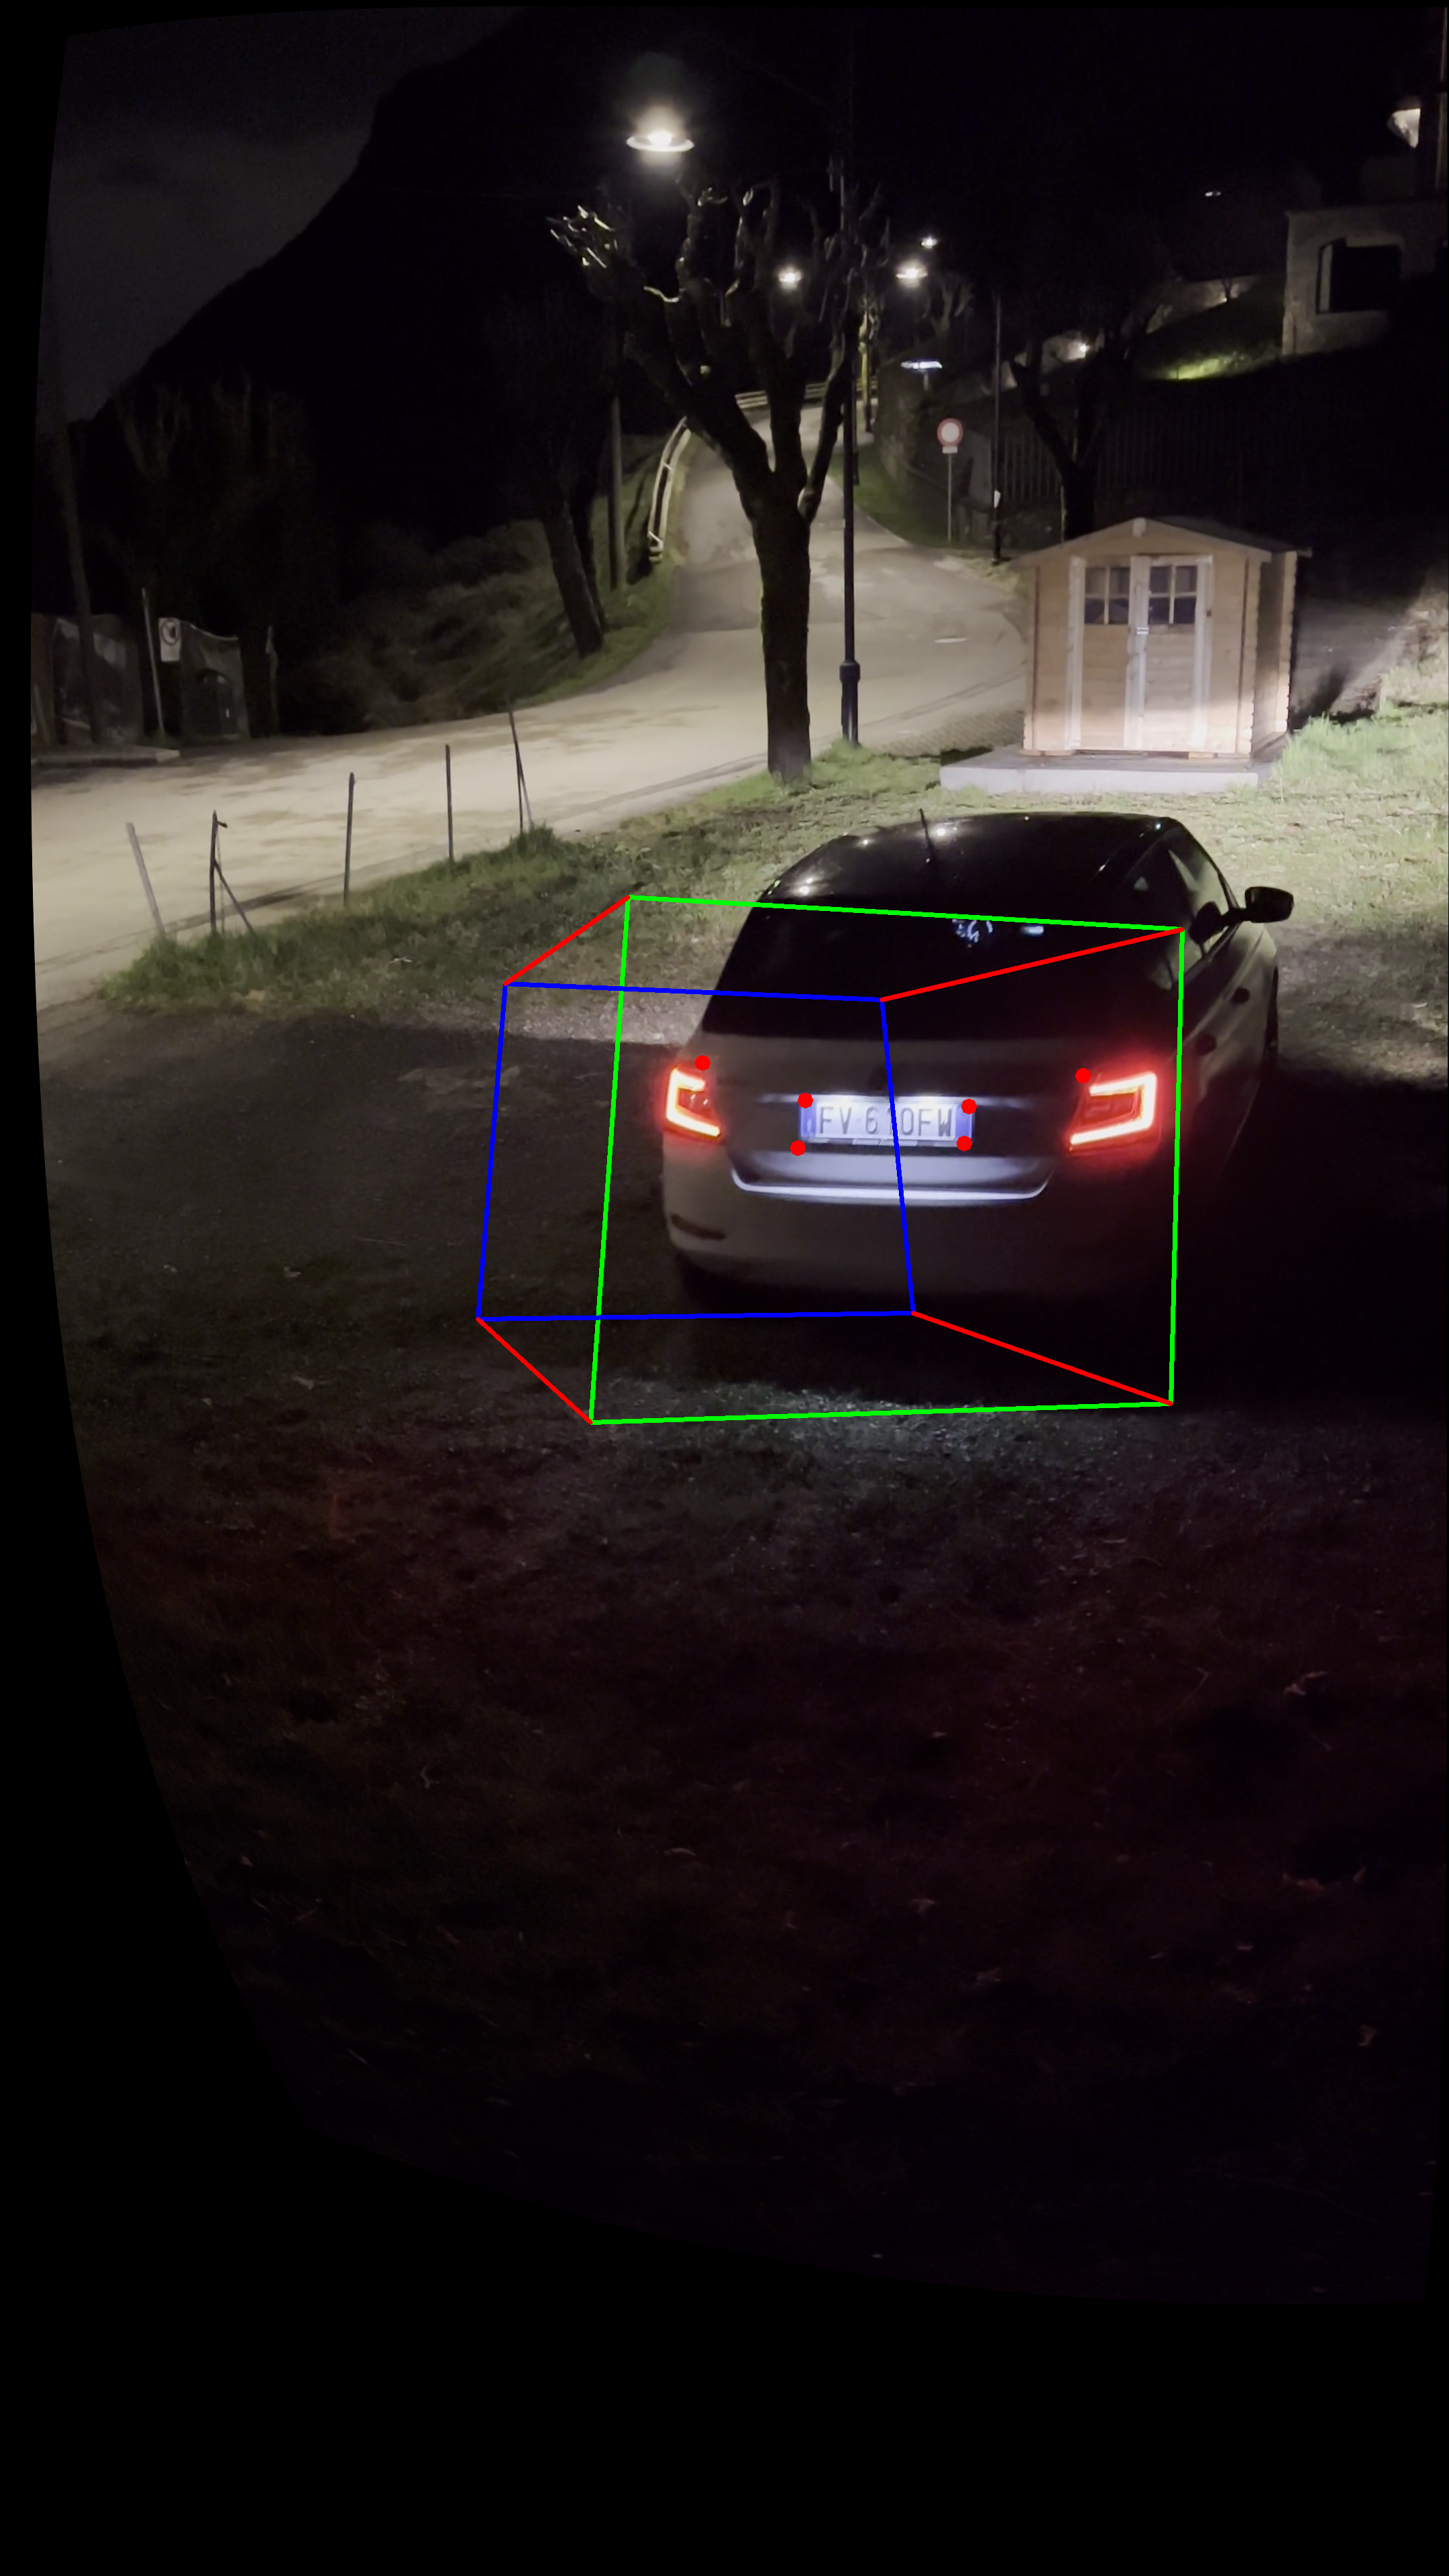
\includegraphics[width=\textwidth]{Images/method4/bbox_4pts_iterative.jpg}
        \caption{4-point PnP using Iterative solver}
    \end{subfigure}
    \hfill
    \begin{subfigure}[b]{0.30\textwidth}
        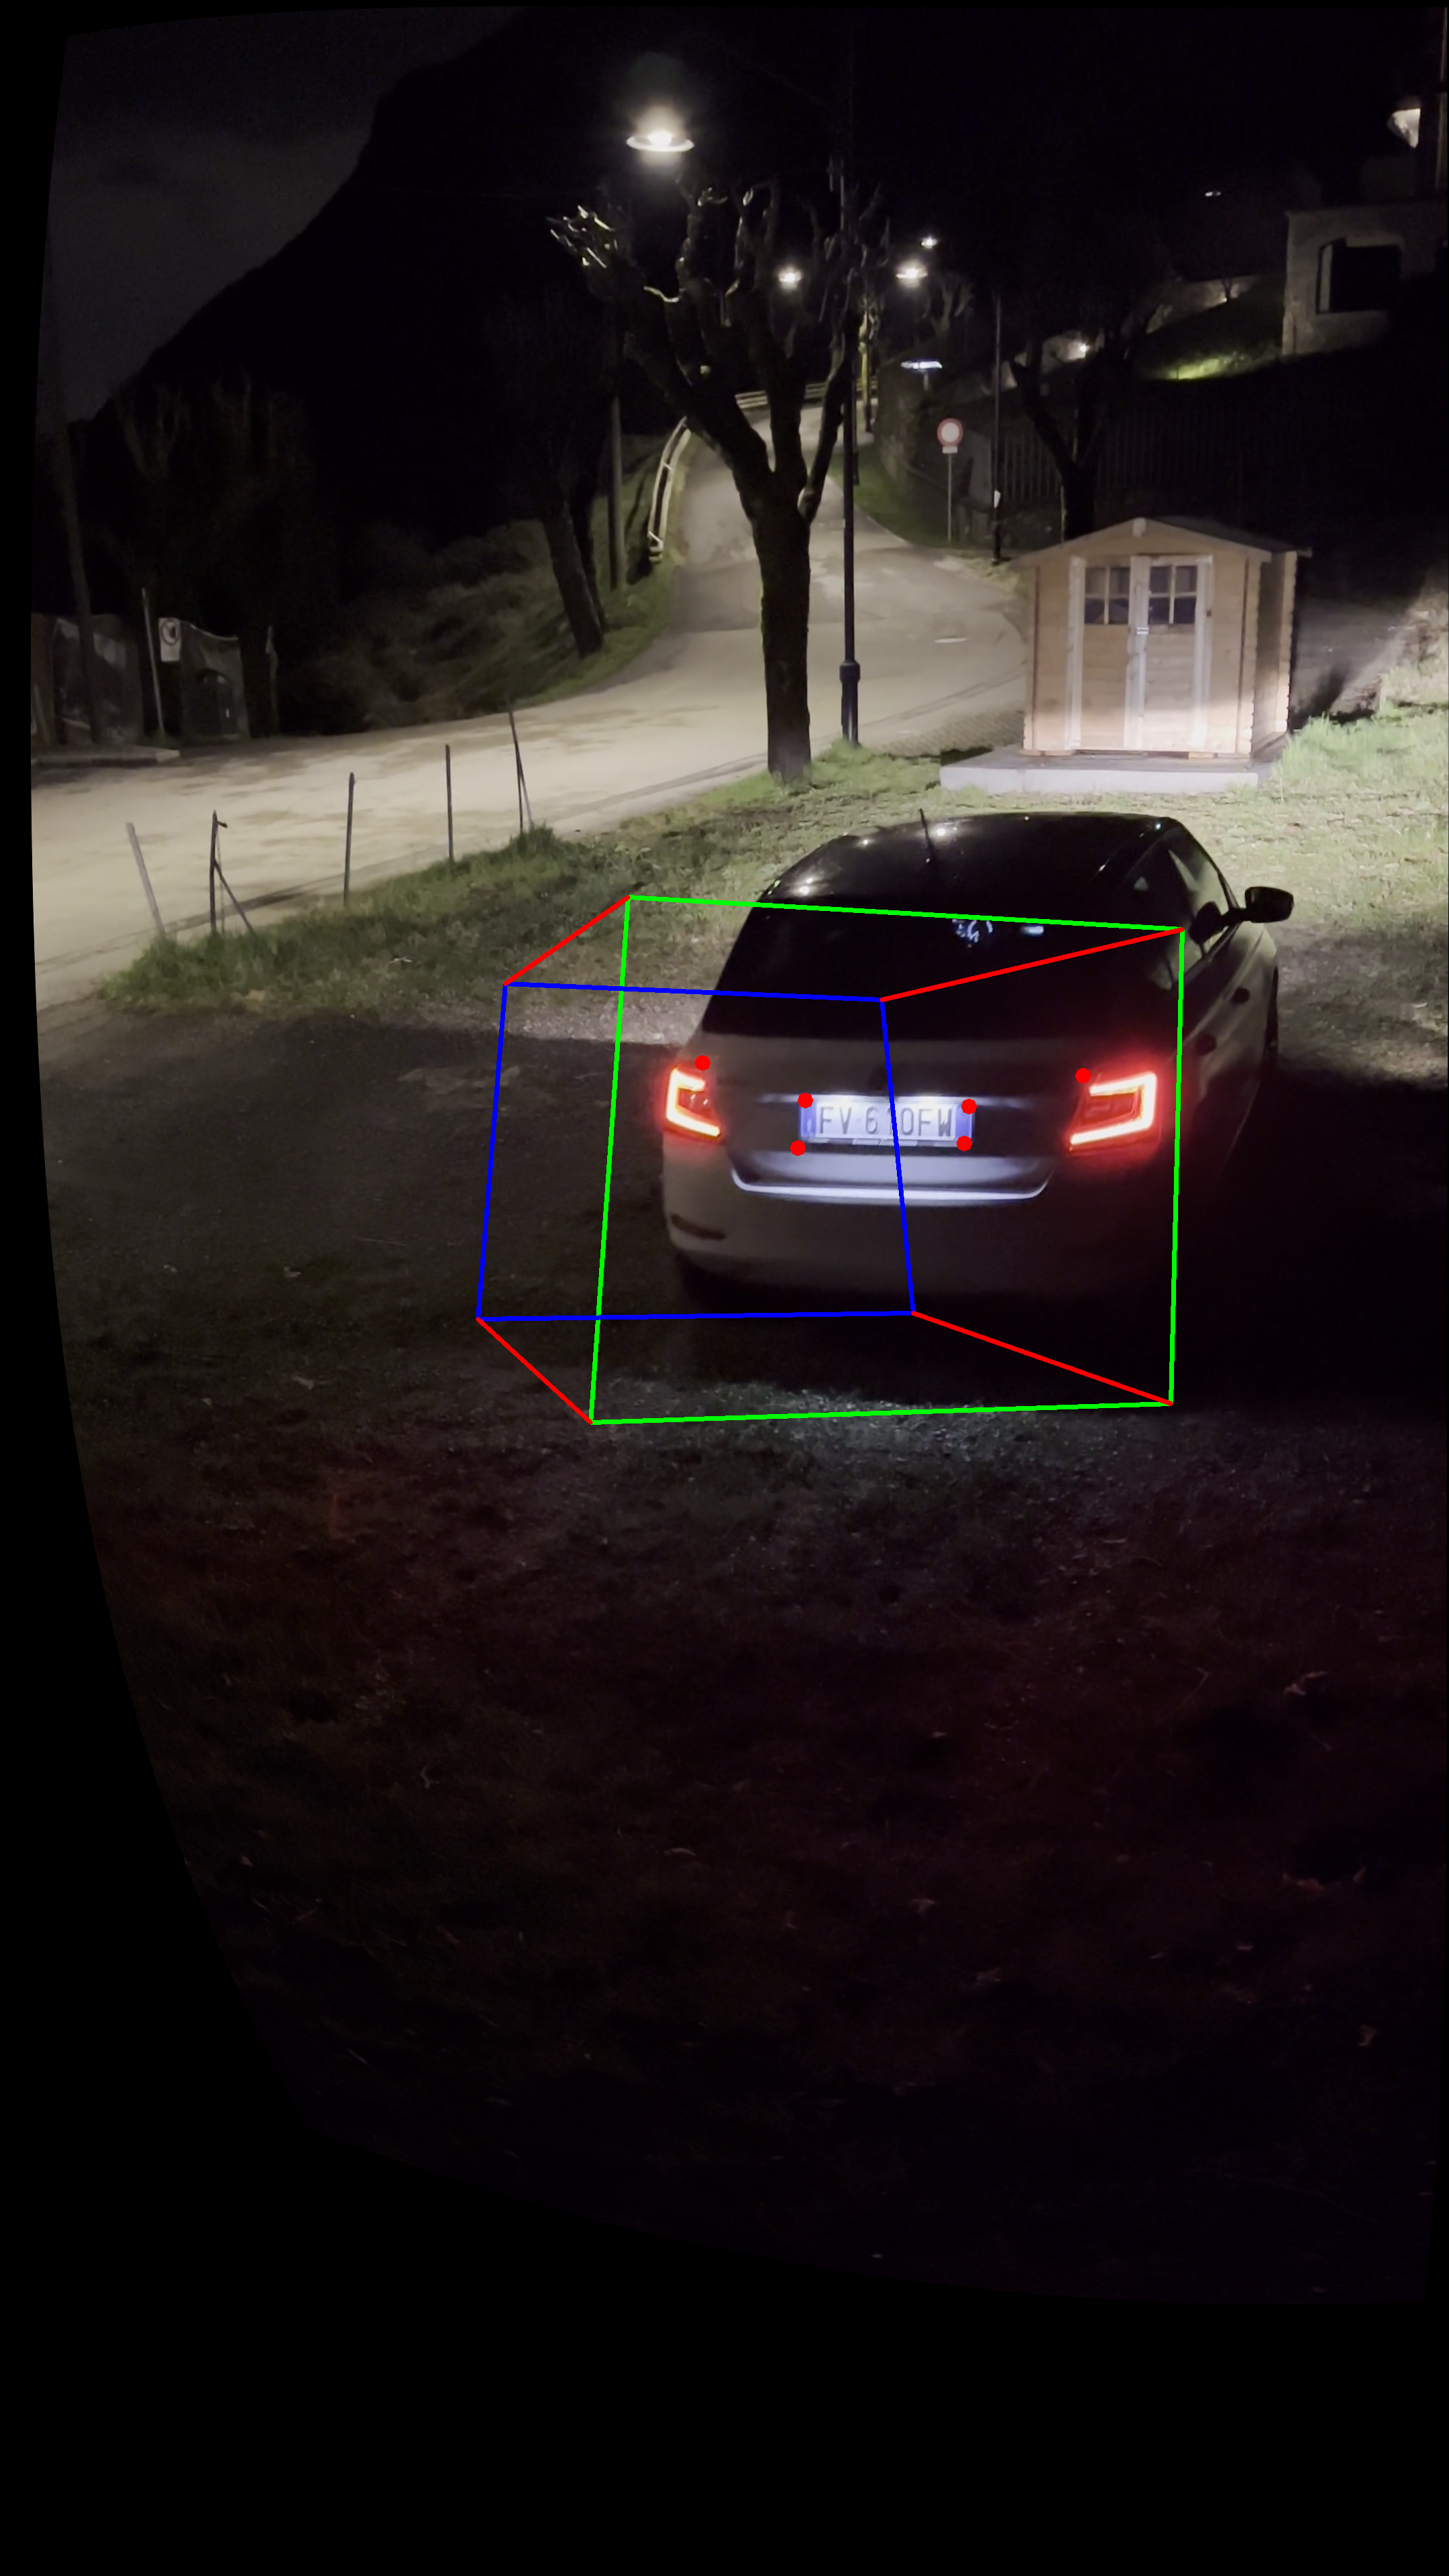
\includegraphics[width=\textwidth]{Images/method4/bbox_4pts_epnp.jpg}
        \caption{4-point PnP using EPnP solver}
    \end{subfigure}
    \hspace*{\fill}
    \caption{Pose estimation comparison using four points and different PnP solvers}
    \label{fig:pnp_4pts}
\end{figure}

Figure~\ref{fig:method4_result} shows the result obtained by extending the model with a fifth point corresponding to the vehicle’s side mirror. The projected bounding box exhibits greater accuracy and spatial consistency, especially in the horizontal extent, validating the benefit of including out-of-plane points in the PnP setup.

\begin{figure}[h]
    \centering
    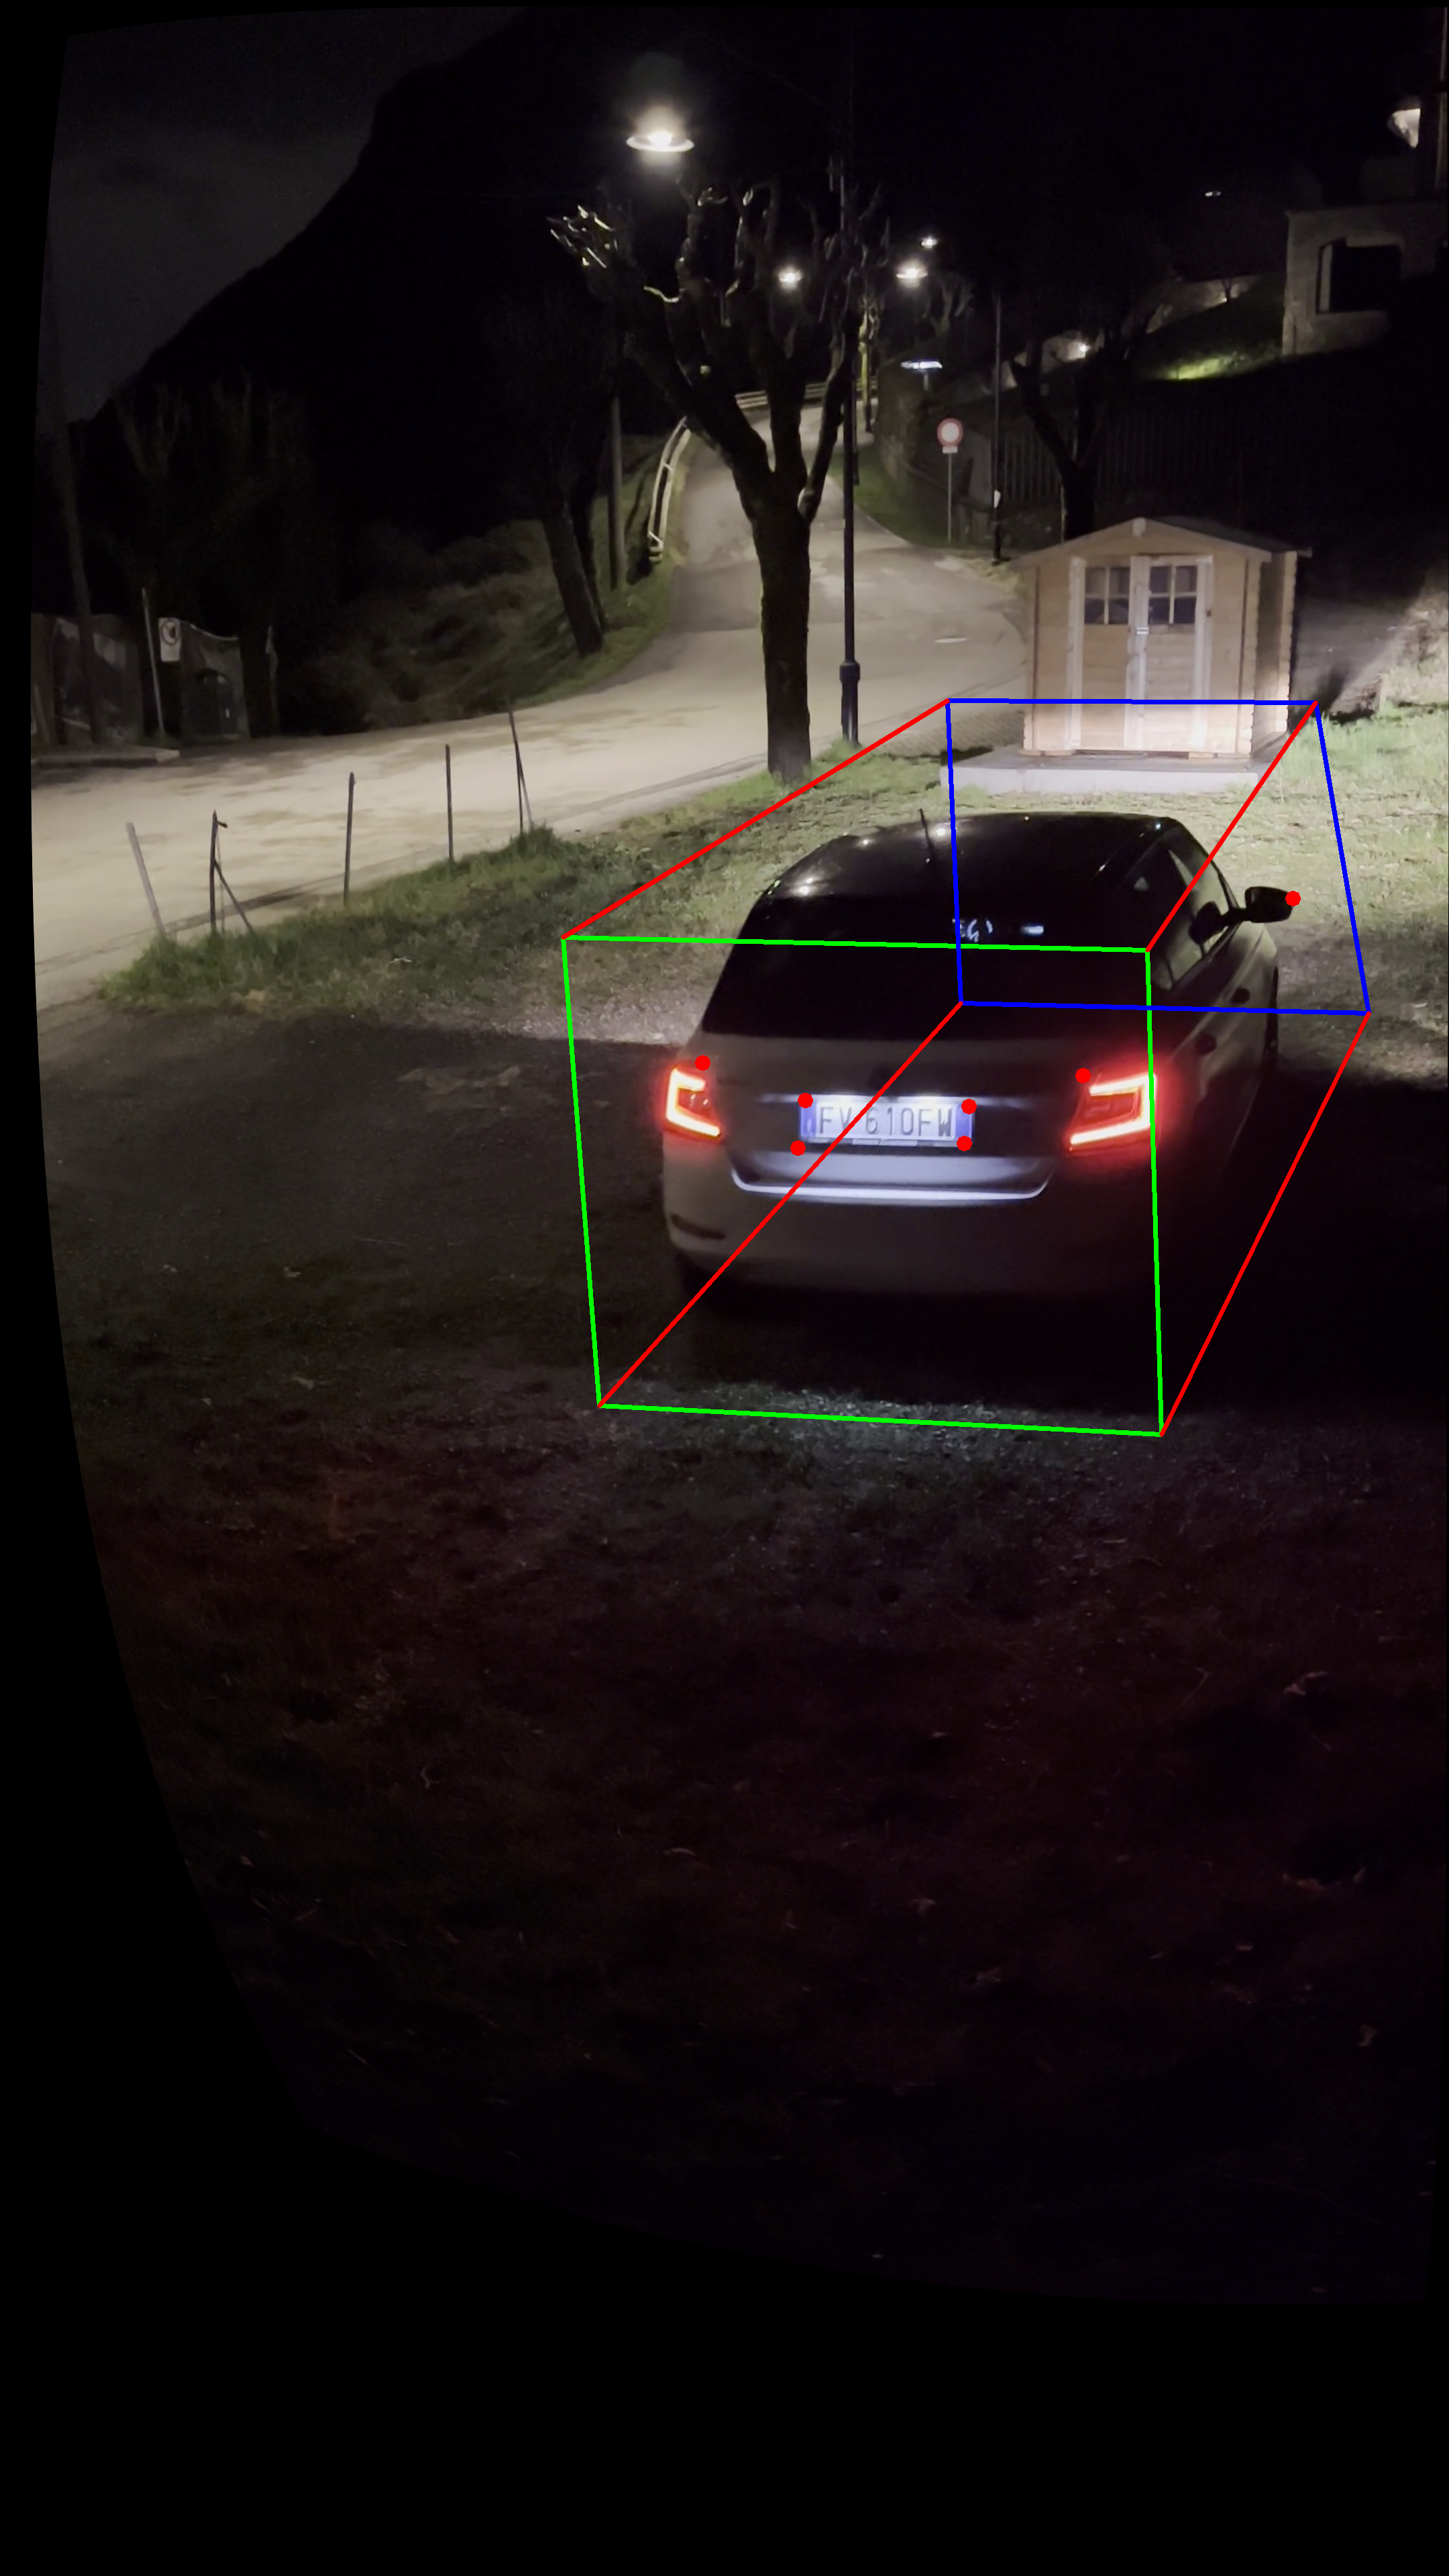
\includegraphics[width=0.35\textwidth]{Images/method4/bbox_5pts_iterative.jpg}
    \caption{Pose estimation using five-point model (license plate, headlights, and mirror)}
    \label{fig:method4_result}
\end{figure}
